\documentclass[12pt]{article}
% controlling the geometry of the page:
\usepackage[margin=1in, paperwidth=8.5in, paperheight=11in]{geometry} 
\usepackage{amsmath, amssymb} % useful math symbols and environments

\usepackage{multicol} % multiple columns side-by-side

\usepackage{amsthm} % Theorem-like environments
\theoremstyle{definition} % Without this line, theorem statements (and therefore problem statements etc.) show up in italic text.
\newtheorem{conjecture}{Conjecture}
\newtheorem{problem}{Problem}
\newtheorem*{remark}{Remark}
\newtheorem*{definition}{Definition}

% pretty colors!
\usepackage[dvipsnames]{xcolor}
\colorlet{darkgrey}{black!70}
\colorlet{darkgreen}{green!50!black}


\usepackage{tikz} % for drawing diagrams
\usetikzlibrary{arrows,automata,positioning} 
\usetikzlibrary{decorations.markings}
\usetikzlibrary{decorations.pathreplacing}
\usetikzlibrary{patterns}
\usetikzlibrary{shapes.geometric}

%%---------------------------------------------------------------------------
%% included from visualalgebra.sty (see the beamer folder)
%% TEXT COLORS
%%
\definecolor{xRed}{rgb}{.9,0,0}       
\definecolor{xBlue}{rgb}{0,0,.9}      
\definecolor{xGreen}{HTML}{009000}   %% "Islamic green"
\definecolor{xPurple}{HTML}{D14FFF}  
\definecolor{xOrange}{HTML}{F56600}  %% "Clemson orange"

\newcommand{\Alert}[1]{\textcolor{xRed}{#1}}
\newcommand{\Balert}[1]{\textcolor{xBlue}{#1}}
\newcommand{\Galert}[1]{\textcolor{xGreen}{#1}}
\newcommand{\Palert}[1]{\textcolor{xPurple}{#1}}
\newcommand{\Oalert}[1]{\textcolor{xOrange}{#1}}
\newcommand{\Walert}[1]{\textcolor{white}{#1}}

%% vertices in cayley graphs
\tikzset{v/.style={circle, draw, fill=lightgray,inner sep=0pt, 
  minimum size=6mm}}

%% Edge colors
%%
\definecolor{eRed}{rgb}{1,0,0}      % Cayley diagram edges
\definecolor{eBlue}{rgb}{0,0,1}     % Cayley diagram edges
\definecolor{eGreen}{HTML}{7EC636}  % Goodnotes green (a little darker)
\definecolor{eGreen}{HTML}{3CAC13}  % I like this a litte better
\definecolor{ePurple}{HTML}{D287FF} % Close to goodnotes 
\colorlet{eOrange}{orange}

% Edge styles 
%%
\tikzset{r/.style={draw, very thick, eRed, -stealth}}  % Red -->
\tikzset{rr/.style={draw, very thick, eRed}}           % Red ---
\tikzset{r2/.style={draw, very thick, eRed,stealth'-stealth'}} % Red <-->
\tikzset{b/.style={draw, very thick, eBlue, -stealth}} % Blue -->
\tikzset{bb/.style={draw, very thick, eBlue}}          % Blue ---
\tikzset{b2/.style={draw, very thick, eBlue,stealth'-stealth'}} % Blue <-->
\tikzset{g/.style={draw, very thick, eGreen, -stealth}} % Green -->
\tikzset{gg/.style={draw, very thick, eGreen}}          % Green ---
\tikzset{g2/.style={draw, very thick, eGreen,stealth'-stealth'}} % Green <-->
\tikzset{p/.style={draw, very thick, ePurple, -stealth}} % Purple -->
\tikzset{pp/.style={draw, very thick, ePurple}}           % Purple ---
\tikzset{p2/.style={draw, very thick, ePurple,stealth'-stealth'}} % Purple <-->
\tikzset{o/.style={draw, very thick, eOrange, -stealth}} % Orange -->
\tikzset{oo/.style={draw, very thick, eOrange}}           % Orange ---
\tikzset{o2/.style={draw, very thick, eOrange,stealth'-stealth'}} % Orange <-->
%%
\tikzstyle{cy2} = [draw,very thick]           %% cycle graph edges
\definecolor{faded}{rgb}{.75,.75,.75}
\tikzstyle{f} = [faded]                         % This is used all the time
%%---------------------------------------------------------------------------
%%
%% COLORS FOR COSET BUBBBLES 
%%
\colorlet{cosetGray}{gray!15!white}
\colorlet{cosetBlue}{blue!15!white}
\colorlet{cosetRed}{red!15!white}
\definecolor{cosetPurple}{rgb}{.9 .84 .965}
\definecolor{cosetGreen}{rgb}{.863 .92 .855}
%%---------------------------------------------------------------------------

\usepackage{graphicx} % for inserting figures with \includegraphics
\usepackage{setspace} % for controlling space between lines, paragraphs, etc.

\usepackage{fancyhdr} % for controlling headers and footers
\usepackage{newtx} % changes the default font family
\usepackage[shortlabels]{enumitem} % controllable labels for ordered and unordered lists

\usepackage{hyperref} % controls hyperlinks, both internal and external
\hypersetup{
    colorlinks=true,
    urlcolor=blue,
}

\setlength{\headheight}{14.5pt}
\newcommand{\Q}{\mathbb{Q}}
\newcommand{\R}{\mathbb{R}}
\newcommand{\Z}{\mathbb{Z}}
\newcommand\inv{^{-1}} % I am very tired of typing ^{-1}
\def\<{\langle}
\def\>{\rangle}
\DeclareMathOperator\Rect{\mathbf{Rect}}
\DeclareMathOperator\Tri{\mathbf{Tri}}
\DeclareMathOperator\Sq{\mathbf{Sq}}
\DeclareMathOperator\Light{\mathbf{Light}}
\DeclareMathOperator{\lcm}{lcm}
%% Abstract algebra commands
\def\normal{\lhd}
\def\normaleq{\unlhd}
\def\nnormal{\ntriangleleft}
\def\nnormaleq{\ntrianglelefteq}

\newenvironment{red}{\color{red}}{\ignorespacesafterend}

% I don't like how LaTeX renders section headings by default
\renewcommand{\section}[1]{\begin{center} \textbf{#1} \\\end{center}}
%
\setlength{\parindent}{0in}
%\oddsidemargin=-.25in
\allowdisplaybreaks
\pagestyle{fancy}
\renewcommand{\headrulewidth}{0pt}
\lhead{MATH 312}
\rhead{Spring 2025}
%\lfoot{\copyright\ CLEAR Calculus 2010}
\cfoot{}
\renewcommand{\thefootnote}{*} 
\hyphenpenalty=10000 % LaTeX by default really likes hyphenating things

% all the stuff above this line is called the preamble...
%##################################################################
\begin{document} % this is always the first line of what's actually produced
\section{Homework \#7 (due Mar 9)} % notice that if you want the character # to appear, you have to "escape" it with a backslash

\begin{definition}
    Let $H \leq G$. The set $G/H$ (we say ``$G$ mod $H$'') is the set of (left) cosets of $H$ in $G$: 
    \[G/H = \{H, aH, bH, \ldots\}\]
    If $H\normaleq G$, then $G/H$ becomes a group if we define the binary operation as
    \[aH \ast bH := (a\ast b)H\]
\end{definition}

%%======================================================================
\subsection*{Elements of quotient groups are cosets}

Do \Alert{a few of} Problems \ref{elements} and \ref{orders}. How many is \Alert{``a few''}? Idk. Make sure you do some that are written additively and some that are written multiplicatively. Part (j) is slightly harder but as a hint it is something we've seen before, perhapst in Homework 5? Hmmm

\begin{problem}\label{elements}
    List out all the elements of the following quotient groups. (I promise that we're taking the quotient by a normal subgroup; no need to check.)
    \begin{multicols}{2}
        \begin{enumerate}[(a)]
            \item $D_4 / \< r \>$
            \item $D_4 / \< r^2 \>$
            \item $\Z / 4\Z$
            \item $Q_8 / \< -1 \>$
            \item $Q_8 / \< k \>$
            \item $\Z_6 / \< 3 \>$
            \item $\Z_6 / \< 2 \>$
            \item $(\Z_3 \times \Z_6) / \< (1, 1) \>$
            \item $(\Z_4 \times \Z_8) / \< (0 ,2) \>$
            \item $A_4 / \<(12)(34), (13)(24)\>$
        \end{enumerate}
    \end{multicols}
\end{problem}

\begin{problem}
    While working on the previous problem, you may have conjectured this: Let $G$ be a group and $H \normaleq G$. Then $|G/H| = [G:H]$. 
    In particular, if $G$ is finite, then $|G/H| = |G| / |H|$.
\end{problem}

\begin{problem}\label{orders}
    Find the order of the given element in the quotient group. (Again, I promise we're taking the quotient by a normal subgroup.)
    \begin{multicols}{2}
        \begin{enumerate}[(a)]
            \item $f\<r\> \in D_4 / \< r \>$
            \item $r\<r^2\> \in D_4 / \< r^2 \>$
            \item $3+4\Z \in \Z / 4\Z$
            \item $j\<-1\> \in Q_8 / \< -1 \>$
            \item $i\<k\> \in Q_8 / \< k \>$
            \item $5 + \<3\> \in \Z_6 / \< 3 \>$
            \item $5 + \<2\> \in \Z_6 / \< 2 \>$
            \item $(2, 1) + \< (1, 1) \> \in (\Z_3 \times \Z_6) / \< (1, 1) \>$
            \item $(1, 3) + \< (0 ,2) \> \in (\Z_4 \times \Z_8) / \< (0 ,2) \>$
            \item $(123) \<(12)(34), (13)(24)\> \\
            \phantom{.}\qquad \in A_4 / \<(12)(34), (13)(24)\>$
        \end{enumerate}
    \end{multicols}
\end{problem}

\begin{problem}
    $\Q$ is an abelian group under addition, so all its subgroups are normal. Describe the quotient group $\Q / \<-1\>$. In particular, what do the elements look like?
\end{problem}

\begin{problem}
    If you take $\Q$ and throw away 0, then what's left is called $\Q^*$, and it is an abelian group under multiplication. Describe the quotient group $\Q^* / \<-1\>$. In particular, what do the elements look like?
\end{problem}

\pagebreak
%%======================================================================
\subsection*{Quotient groups are visible in subgroup lattices}

\begin{problem} Consider $Q_8 / \<-1\>$, which I am tired of typing and will therefore just call ``$Q$''.
    \begin{enumerate}[(a)]
        \item In Problem \ref{elements}, you found that $Q$ has order 4. There are only two possible groups of order 4; is $Q \cong C_4$ or is $Q \cong V_4$? How do you know?
        \item Draw the subgroup lattice of $Q$.
        \item Where can you find the subgroup lattice of $Q$ inside the subgroup lattice of $Q_8$?
    \end{enumerate}
    \[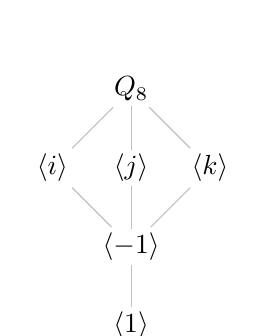
\begin{tikzpicture}
        \begin{scope}[shorten >= -2pt,shorten <= -2pt]
            \node(Q8) at (0,3) {$Q_8$};
            \node(i) at (-1,2) { $\<i\>$};
            \node(j) at (0,2) { $\<j\>$};
            \node(k) at (1,2) { $\<k\>$};
            \node(-1) at (0,1) { $\<-1\>$};
            \node(1) at (0,0) { $\left\<1\right\>$};
            \draw[f](1)--(-1); \draw[f](-1)--(i); \draw[f](-1)--(j); \draw[f](-1)--(k);
            \draw[f](Q8)--(i); \draw[f](Q8)--(j); \draw[f](Q8)--(k);
        \end{scope}
    \end{tikzpicture}\]
\end{problem}

\begin{problem}
    Explore this phenomenon in a bigger and weirder group. LMFDB calls this group $C_3 : C_4$. Group Explorer calls it $\Z_3 \rtimes \Z_4$. It's also called $Q_{12}$ because it is a ``generalized quaternion group.'' (If you look at the subgroup lattice I think you can kinda see why.)
    %% Generalized quaternion group (dicyclic) of order 12.
    \tikzstyle{R6-out} = [draw, very thick, Red,-stealth,bend right=18]
    \tikzstyle{R6-in} = [draw, very thick, Red,-stealth,bend left=12]
    \tikzstyle{R-out} = [draw, very thick, Red,-stealth,bend right=15]
    \tikzstyle{R-in} = [draw, very thick, Red,-stealth,bend left=12]
    \tikzstyle{B} = [draw, very thick, Blue,-stealth,bend right=25]
    \[
    \begin{tikzpicture}[scale=1.25]
        \tikzstyle{v} = [circle, draw, fill=lightgray,inner sep=0pt, 
        minimum size=6.25mm]
        %%
        \begin{scope}[shift={(0,0)}]
            \tikzstyle{every node}=[font=\small]
            \node (1) at (0:2) [v] {$1$};
            \node (r) at (60:2) [v] {$r$};
            \node (r2) at (120:2) [v] {$r^2$};
            \node (r3) at (180:2) [v] {$r^3$};
            \node (r4) at (240:2) [v] {$r^4$};
            \node (r5) at (300:2) [v] {$r^5$};
            \node (s) at (0:1) [v] {$s$};
            \node (sr5) at (60:1) [v] {$rs$};
            \node (sr4) at (120:1) [v] {$r^2\!s$};
            \node (sr3) at (180:1) [v] {$r^3\!s$};
            \node (sr2) at (240:1) [v] {$r^4\!s$};
            \node (sr) at (300:1) [v] {$r^5\!s$};
            %%
            \path[b] (1) to (s);
            \path[B] (s) to (r3);
            \path[b] (r3) to (sr3);
            \path[B] (sr3) to (1);
            %%
            \path[b] (r) to (sr5);
            \path[B] (sr5) to (r4);
            \path[b] (r4) to (sr2);
            \path[B] (sr2) to (r);
            %%
            \path[b] (r2) to (sr4);
            \path[B] (sr4) to (r5);
            \path[b] (r5) to (sr);
            \path[B] (sr) to (r2);
            \path[R6-out] (1) to (r);
            \path[R6-out] (r) to (r2);
            \path[R6-out] (r2) to (r3);
            \path[R6-out] (r3) to (r4);
            \path[R6-out] (r4) to (r5);
            \path[R6-out] (r5) to (1);
            \path[R-in] (sr5) to (s);
            \path[R-in] (sr4) to (sr5);
            \path[R-in] (sr3) to (sr4);
            \path[R-in] (sr2) to (sr3);
            \path[R-in] (sr) to (sr2);
            \path[R-in] (s) to (sr);
        \end{scope}
        \begin{scope}[shift={(5,-2)},shorten >= -2pt,shorten <= -2pt, scale=0.8]
            \node(Q12) at (0,5) {$Q_{12}$};
            \node(r) at (-2, 4) {$\<r\>$};
            \node(s) at (0,3) { $\<s\>$};
            \node(r2s) at (1,3) { $\<r^2\!s\>$};
            \node(r4s) at (2,3) { $\<r^4\!s\>$};
            \node(r2) at (-2, 2) {$\<r^2\>$};
            \node(r3) at (1,1) { $\<r^3\>$};
            \node(1) at (0,0) { $\left\<1\right\>$};
            \draw[f](Q12)--(s); \draw[f](Q12)--(r2s); \draw[f](Q12)--(r4s); 
            \draw[f](Q12)--(r);
            \draw[f](r3)--(s); \draw[f](r3)--(r2s); \draw[f](r3)--(r4s);
            \draw[f](r)--(r2);
            \draw[xPurple](r3)--(r);
            %\draw[xPurple](r3) to [bend left=20](r);
            \draw[f](1)--(r2); \draw[f](1)--(r3);
            \node at (3.5, 5.5) {\textbf{Order}};
            \node at (3.5, 5) {$12$};
            \node at (3.5, 4) {$6$};
            \node at (3.5, 3) {$4$};
            \node at (3.5, 2) {$3$};
            \node at (3.5, 1) {$2$};
            \node at (3.5, 0) {$1$};
        \end{scope}
    \end{tikzpicture}
  \]
  \begin{enumerate}[(a)]
    \item Looking at the subgroup lattice, which subgroups of $Q_{12}$ are normal? How do you know?
    \item List the elements of $Q_{12} / \<r^3\>$, draw a Cayley graph, and draw the subgroup lattice. Where do you see the subgroup lattice of $Q_{12}/\<r^3\>$ inside the subgroup lattice of $Q_{12}$?
    \item (Bonus) Do the same for $Q_{12}/\<r^2\>$.
    \item (Also bonus) Calculating with presentations is fun. Use the presentation \[Q_{12} = \big\< r, s \mid r^6 = 1, s^4 = 1, s^2 = r^3, rs = sr\inv \big\>\] to show that all three of the order-4 subgroups are conjugate.
  \end{enumerate}
\end{problem}

\pagebreak

\subsection*{Interesting facts about quotient groups}

\begin{problem}\label{abqt}
    Let $G$ be a group and let $H\normaleq G$. Show that if $G$ is abelian, then so is $G/H$.
\end{problem}

\begin{problem}\label{cyqt}
    Let $G$ be a group and let $H\normaleq G$. Show that if $G$ is cyclic, then so is $G/H$.
\end{problem}

\begin{problem}\label{zqt}
    We previously proved that $Z(G) \normaleq G$. Show that if $G/Z(G)$ is cyclic, then $G$ is abelian.

    Progressively hinty hints (decode at rot13.com):
    \begin{itemize}
        \item Gur pbfrgf bs n fhotebhc cnegvgvba gur tebhc.
        \item Jung qb gur pbfrgf bs M(T) ybbx yvxr?
        \item Fnl T/M(T) vf trarengrq ol tM(T). Nal ryrzrag k va T unf gb yvir va bar bs gur pbfrgf bs M(T).
        \item Fnl T/M(T) vf trarengrq ol tM(T). Fubj gung nal ryrzrag k va T vf fbzr cbjre bs t zhygvcyvrq ol fbzr ryrzrag bs M(T).
    \end{itemize}
\end{problem}

\begin{problem}[Bonus]
    Is the converse of Problem \ref{abqt} true? Prove it, or find a specific counterexample.
\end{problem}

\begin{problem}[Bonus]
    Is the converse of Problem \ref{cyqt} true? Prove it, or find a specific counterexample.
\end{problem}

\begin{problem}[Bonus]
    Is the converse of Problem \ref{zqt} true? Prove it, or find a specific counterexample.
\end{problem}

\begin{problem}[Andrew]
    Prove that $\Z/n\Z$ is cyclic of order $n$.

    Another way to say this is the following useful fact: $\Z/n\Z \cong \Z_n$.

    (This is actually a special case of Problem \ref{cyqt}.)
\end{problem}

\end{document}

